\documentclass{article}
\usepackage[margin=1in]{geometry}
\usepackage{tikz}
\usetikzlibrary{positioning,arrows.meta,fit,backgrounds,calc}
\usepackage{tcolorbox}
\usepackage{fontawesome5}
\usepackage{xcolor}

\newcommand{\benchmark}{ChemChain}

\begin{document}

\begin{figure}[t]
    \centering

    % VERSION 3: Grouped Reactions with Stage Boxes
    \begin{tcolorbox}[
        title=\textbf{Chemistry: Reaction Cascade} \hfill {\small\colorbox{teal!20}{Medium} \quad 9 steps},
        colframe=teal!70!black,
        colback=teal!3,
        boxrule=0.8pt,
        width=\textwidth
    ]
    \small
    \begin{tikzpicture}[remember picture, overlay]
        \node[opacity=0.05, anchor=east] at ([xshift=-0.4cm, yshift=0.15cm]current page.east) {\Huge\faFlask};
    \end{tikzpicture}

    \textbf{Reaction pathway:}
    \begin{center}
    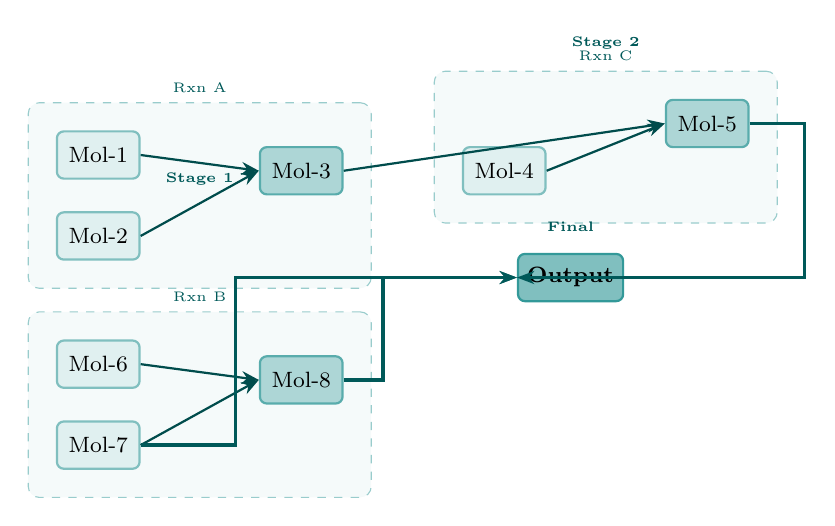
\begin{tikzpicture}[
        node distance=0.7cm and 1.0cm,
        mol/.style={draw, rounded corners=2.5pt, minimum width=1.05cm, minimum height=0.6cm, thick, font=\footnotesize},
        substrate/.style={mol, fill=teal!12, draw=teal!50},
        product/.style={mol, fill=teal!32, draw=teal!65},
        final/.style={mol, fill=teal!50, draw=teal!80, font=\footnotesize\bfseries},
        stage/.style={draw=teal!40, fill=teal!4, rounded corners=4pt, dashed, inner sep=0.35cm},
        arrow/.style={-{Stealth[length=2.2mm]}, very thick, teal!70!black},
        combine/.style={-{Stealth[length=2.2mm]}, thick, teal!60!black}
    ]
        % Stage 1: Parallel reactions
        \node[substrate] (m1) {Mol-1};
        \node[substrate, below=0.4cm of m1] (m2) {Mol-2};
        \node[product, right=1.5cm of m1.east, yshift=-0.2cm] (m3) {Mol-3};
        \draw[combine] (m1.east) -- (m3.west);
        \draw[combine] (m2.east) -- (m3.west);

        \node[substrate, below=1.0cm of m2] (m6) {Mol-6};
        \node[substrate, below=0.4cm of m6] (m7) {Mol-7};
        \node[product, right=1.5cm of m6.east, yshift=-0.2cm] (m8) {Mol-8};
        \draw[combine] (m6.east) -- (m8.west);
        \draw[combine] (m7.east) -- (m8.west);

        % Stage boxes
        \begin{scope}[on background layer]
            \node[stage, fit=(m1)(m2)(m3), label={[font=\tiny, teal!70!black]above:Rxn A}] (stage1a) {};
            \node[stage, fit=(m6)(m7)(m8), label={[font=\tiny, teal!70!black]above:Rxn B}] (stage1b) {};
        \end{scope}

        % Stage 2: Second combination
        \node[substrate, right=1.5cm of m3] (m4) {Mol-4};
        \node[product, right=1.5cm of m4.east, yshift=0.6cm] (m5) {Mol-5};
        \draw[combine] (m3.east) -- (m5.west);
        \draw[combine] (m4.east) -- (m5.west);

        \begin{scope}[on background layer]
            \node[stage, fit=(m4)(m5), label={[font=\tiny, teal!70!black]above:Rxn C}] (stage2) {};
        \end{scope}

        % Final stage: Output
        \node[final, right=2.2cm of m8.east, yshift=1.3cm] (out) {Output};
        \draw[arrow] (m5.east) -| ([xshift=0.7cm]m5.east) |- (out.west);
        \draw[arrow] (m8.east) -| ([xshift=0.5cm]m8.east) |- (out.west);
        \draw[arrow] (m7.east) -| ([xshift=1.2cm]m7.east) |- (out.west);

        % Stage labels
        \node[font=\tiny\bfseries, teal!70!black, anchor=south] at ($(stage1a.north)!0.5!(stage1b.north) + (0,0.15)$) {Stage 1};
        \node[font=\tiny\bfseries, teal!70!black, anchor=south] at ($(stage2.north) + (0,0.15)$) {Stage 2};
        \node[font=\tiny\bfseries, teal!70!black, anchor=south] at ($(out.north) + (0,0.15)$) {Final};
    \end{tikzpicture}
    \end{center}

    \vspace{-0.1cm}
    \begin{tabular}{@{}p{0.48\textwidth}p{0.48\textwidth}@{}}
    \textit{Sample step (Subproblem 3):} React Mol-1 + Mol-2 in THF at room temp. Predict major product. &
    \textit{Final step:} Count hydrogens in Mol-5, Mol-7, Mol-8. \\
    \end{tabular}

    \vspace{0.2cm}
    \hfill \textbf{Answer:} \texttt{[19, 15, 23]}
    \end{tcolorbox}

    \caption{\textbf{Version 3:} Grouped layout showing parallel reactions in Stage 1 (Rxn A \& B), sequential reaction in Stage 2 (Rxn C), and final combination. Dashed boxes group related reaction steps.}
\end{figure}

\end{document}
